%% template.tex
%% from
%% bare_conf.tex
%% V1.4b
%% 2015/08/26
%% by Michael Shell
%% See:
%% http://www.michaelshell.org/
%% for current contact information.
%%
%% This is a skeleton file demonstrating the use of IEEEtran.cls
%% (requires IEEEtran.cls version 1.8b or later) with an IEEE
%% conference paper.
%%
%% Support sites:
%% http://www.michaelshell.org/tex/ieeetran/
%% http://www.ctan.org/pkg/ieeetran
%% and
%% http://www.ieee.org/

%%*************************************************************************
%% Legal Notice:
%% This code is offered as-is without any warranty either expressed or
%% implied; without even the implied warranty of MERCHANTABILITY or
%% FITNESS FOR A PARTICULAR PURPOSE!
%% User assumes all risk.
%% In no event shall the IEEE or any contributor to this code be liable for
%% any damages or losses, including, but not limited to, incidental,
%% consequential, or any other damages, resulting from the use or misuse
%% of any information contained here.
%%
%% All comments are the opinions of their respective authors and are not
%% necessarily endorsed by the IEEE.
%%
%% This work is distributed under the LaTeX Project Public License (LPPL)
%% ( http://www.latex-project.org/ ) version 1.3, and may be freely used,
%% distributed and modified. A copy of the LPPL, version 1.3, is included
%% in the base LaTeX documentation of all distributions of LaTeX released
%% 2003/12/01 or later.
%% Retain all contribution notices and credits.
%% ** Modified files should be clearly indicated as such, including  **
%% ** renaming them and changing author support contact information. **
%%*************************************************************************


% *** Authors should verify (and, if needed, correct) their LaTeX system  ***
% *** with the testflow diagnostic prior to trusting their LaTeX platform ***
% *** with production work. The IEEE's font choices and paper sizes can   ***
% *** trigger bugs that do not appear when using other class files.       ***                          ***
% The testflow support page is at:
% http://www.michaelshell.org/tex/testflow/

\documentclass[conference,final,]{IEEEtran}
% Some Computer Society conferences also require the compsoc mode option,
% but others use the standard conference format.
%
% If IEEEtran.cls has not been installed into the LaTeX system files,
% manually specify the path to it like:
% \documentclass[conference]{../sty/IEEEtran}





% Some very useful LaTeX packages include:
% (uncomment the ones you want to load)


% *** MISC UTILITY PACKAGES ***
%
%\usepackage{ifpdf}
% Heiko Oberdiek's ifpdf.sty is very useful if you need conditional
% compilation based on whether the output is pdf or dvi.
% usage:
% \ifpdf
%   % pdf code
% \else
%   % dvi code
% \fi
% The latest version of ifpdf.sty can be obtained from:
% http://www.ctan.org/pkg/ifpdf
% Also, note that IEEEtran.cls V1.7 and later provides a builtin
% \ifCLASSINFOpdf conditional that works the same way.
% When switching from latex to pdflatex and vice-versa, the compiler may
% have to be run twice to clear warning/error messages.






% *** CITATION PACKAGES ***
%
%\usepackage{cite}
% cite.sty was written by Donald Arseneau
% V1.6 and later of IEEEtran pre-defines the format of the cite.sty package
% \cite{} output to follow that of the IEEE. Loading the cite package will
% result in citation numbers being automatically sorted and properly
% "compressed/ranged". e.g., [1], [9], [2], [7], [5], [6] without using
% cite.sty will become [1], [2], [5]--[7], [9] using cite.sty. cite.sty's
% \cite will automatically add leading space, if needed. Use cite.sty's
% noadjust option (cite.sty V3.8 and later) if you want to turn this off
% such as if a citation ever needs to be enclosed in parenthesis.
% cite.sty is already installed on most LaTeX systems. Be sure and use
% version 5.0 (2009-03-20) and later if using hyperref.sty.
% The latest version can be obtained at:
% http://www.ctan.org/pkg/cite
% The documentation is contained in the cite.sty file itself.






% *** GRAPHICS RELATED PACKAGES ***
%
\ifCLASSINFOpdf
  % \usepackage[pdftex]{graphicx}
  % declare the path(s) where your graphic files are
  % \graphicspath{{../pdf/}{../jpeg/}}
  % and their extensions so you won't have to specify these with
  % every instance of \includegraphics
  % \DeclareGraphicsExtensions{.pdf,.jpeg,.png}
\else
  % or other class option (dvipsone, dvipdf, if not using dvips). graphicx
  % will default to the driver specified in the system graphics.cfg if no
  % driver is specified.
  % \usepackage[dvips]{graphicx}
  % declare the path(s) where your graphic files are
  % \graphicspath{{../eps/}}
  % and their extensions so you won't have to specify these with
  % every instance of \includegraphics
  % \DeclareGraphicsExtensions{.eps}
\fi
% graphicx was written by David Carlisle and Sebastian Rahtz. It is
% required if you want graphics, photos, etc. graphicx.sty is already
% installed on most LaTeX systems. The latest version and documentation
% can be obtained at:
% http://www.ctan.org/pkg/graphicx
% Another good source of documentation is "Using Imported Graphics in
% LaTeX2e" by Keith Reckdahl which can be found at:
% http://www.ctan.org/pkg/epslatex
%
% latex, and pdflatex in dvi mode, support graphics in encapsulated
% postscript (.eps) format. pdflatex in pdf mode supports graphics
% in .pdf, .jpeg, .png and .mps (metapost) formats. Users should ensure
% that all non-photo figures use a vector format (.eps, .pdf, .mps) and
% not a bitmapped formats (.jpeg, .png). The IEEE frowns on bitmapped formats
% which can result in "jaggedy"/blurry rendering of lines and letters as
% well as large increases in file sizes.
%
% You can find documentation about the pdfTeX application at:
% http://www.tug.org/applications/pdftex





% *** MATH PACKAGES ***
%
%\usepackage{amsmath}
% A popular package from the American Mathematical Society that provides
% many useful and powerful commands for dealing with mathematics.
%
% Note that the amsmath package sets \interdisplaylinepenalty to 10000
% thus preventing page breaks from occurring within multiline equations. Use:
%\interdisplaylinepenalty=2500
% after loading amsmath to restore such page breaks as IEEEtran.cls normally
% does. amsmath.sty is already installed on most LaTeX systems. The latest
% version and documentation can be obtained at:
% http://www.ctan.org/pkg/amsmath





% *** SPECIALIZED LIST PACKAGES ***
%
%\usepackage{algorithmic}
% algorithmic.sty was written by Peter Williams and Rogerio Brito.
% This package provides an algorithmic environment fo describing algorithms.
% You can use the algorithmic environment in-text or within a figure
% environment to provide for a floating algorithm. Do NOT use the algorithm
% floating environment provided by algorithm.sty (by the same authors) or
% algorithm2e.sty (by Christophe Fiorio) as the IEEE does not use dedicated
% algorithm float types and packages that provide these will not provide
% correct IEEE style captions. The latest version and documentation of
% algorithmic.sty can be obtained at:
% http://www.ctan.org/pkg/algorithms
% Also of interest may be the (relatively newer and more customizable)
% algorithmicx.sty package by Szasz Janos:
% http://www.ctan.org/pkg/algorithmicx




% *** ALIGNMENT PACKAGES ***
%
%\usepackage{array}
% Frank Mittelbach's and David Carlisle's array.sty patches and improves
% the standard LaTeX2e array and tabular environments to provide better
% appearance and additional user controls. As the default LaTeX2e table
% generation code is lacking to the point of almost being broken with
% respect to the quality of the end results, all users are strongly
% advised to use an enhanced (at the very least that provided by array.sty)
% set of table tools. array.sty is already installed on most systems. The
% latest version and documentation can be obtained at:
% http://www.ctan.org/pkg/array


% IEEEtran contains the IEEEeqnarray family of commands that can be used to
% generate multiline equations as well as matrices, tables, etc., of high
% quality.




% *** SUBFIGURE PACKAGES ***
%\ifCLASSOPTIONcompsoc
%  \usepackage[caption=false,font=normalsize,labelfont=sf,textfont=sf]{subfig}
%\else
%  \usepackage[caption=false,font=footnotesize]{subfig}
%\fi
% subfig.sty, written by Steven Douglas Cochran, is the modern replacement
% for subfigure.sty, the latter of which is no longer maintained and is
% incompatible with some LaTeX packages including fixltx2e. However,
% subfig.sty requires and automatically loads Axel Sommerfeldt's caption.sty
% which will override IEEEtran.cls' handling of captions and this will result
% in non-IEEE style figure/table captions. To prevent this problem, be sure
% and invoke subfig.sty's "caption=false" package option (available since
% subfig.sty version 1.3, 2005/06/28) as this is will preserve IEEEtran.cls
% handling of captions.
% Note that the Computer Society format requires a larger sans serif font
% than the serif footnote size font used in traditional IEEE formatting
% and thus the need to invoke different subfig.sty package options depending
% on whether compsoc mode has been enabled.
%
% The latest version and documentation of subfig.sty can be obtained at:
% http://www.ctan.org/pkg/subfig




% *** FLOAT PACKAGES ***
%

%\usepackage{fixltx2e}
% fixltx2e, the successor to the earlier fix2col.sty, was written by
% Frank Mittelbach and David Carlisle. This package corrects a few problems
% in the LaTeX2e kernel, the most notable of which is that in current
% LaTeX2e releases, the ordering of single and double column floats is not
% guaranteed to be preserved. Thus, an unpatched LaTeX2e can allow a
% single column figure to be placed prior to an earlier double column
% figure.
% Be aware that LaTeX2e kernels dated 2015 and later have fixltx2e.sty's
% corrections already built into the system in which case a warning will
% be issued if an attempt is made to load fixltx2e.sty as it is no longer
% needed.
% The latest version and documentation can be found at:
% http://www.ctan.org/pkg/fixltx2e


%\usepackage{stfloats}
% stfloats.sty was written by Sigitas Tolusis. This package gives LaTeX2e
% the ability to do double column floats at the bottom of the page as well
% as the top. (e.g., "\begin{figure*}[!b]" is not normally possible in
% LaTeX2e). It also provides a command:
%\fnbelowfloat
% to enable the placement of footnotes below bottom floats (the standard
% LaTeX2e kernel puts them above bottom floats). This is an invasive package
% which rewrites many portions of the LaTeX2e float routines. It may not work
% with other packages that modify the LaTeX2e float routines. The latest
% version and documentation can be obtained at:
% http://www.ctan.org/pkg/stfloats
% Do not use the stfloats baselinefloat ability as the IEEE does not allow
% \baselineskip to stretch. Authors submitting work to the IEEE should note
% that the IEEE rarely uses double column equations and that authors should try
% to avoid such use. Do not be tempted to use the cuted.sty or midfloat.sty
% packages (also by Sigitas Tolusis) as the IEEE does not format its papers in
% such ways.
% Do not attempt to use stfloats with fixltx2e as they are incompatible.
% Instead, use Morten Hogholm'a dblfloatfix which combines the features
% of both fixltx2e and stfloats:
%
% \usepackage{dblfloatfix}
% The latest version can be found at:
% http://www.ctan.org/pkg/dblfloatfix




% *** PDF, URL AND HYPERLINK PACKAGES ***
%
%\usepackage{url}
% url.sty was written by Donald Arseneau. It provides better support for
% handling and breaking URLs. url.sty is already installed on most LaTeX
% systems. The latest version and documentation can be obtained at:
% http://www.ctan.org/pkg/url
% Basically, \url{my_url_here}.




% *** Do not adjust lengths that control margins, column widths, etc. ***
% *** Do not use packages that alter fonts (such as pslatex).         ***
% There should be no need to do such things with IEEEtran.cls V1.6 and later.
% (Unless specifically asked to do so by the journal or conference you plan
% to submit to, of course. )



%% BEGIN MY ADDITIONS %%


\usepackage{longtable,booktabs}

\usepackage[unicode=true]{hyperref}

\hypersetup{
            pdftitle={Urban and socio-economic correlates of property price evolution:~Application to Dublin's costal area},
            pdfkeywords={Property price, Housing Market, Feature Analysis, Machine Learning, Geocoding},
            pdfborder={0 0 0},
            breaklinks=true}
\urlstyle{same}  % don't use monospace font for urls

% Pandoc toggle for numbering sections (defaults to be off)
\setcounter{secnumdepth}{5}

% Pandoc syntax highlighting


% Pandoc header
\usepackage{graphicx}
\usepackage{booktabs}
\usepackage{longtable}
\usepackage{array}
\usepackage{multirow}
\usepackage{wrapfig}
\usepackage{float}
\usepackage{colortbl}
\usepackage{pdflscape}
\usepackage{tabu}
\usepackage{threeparttable}
\usepackage{threeparttablex}
\usepackage[normalem]{ulem}
\usepackage{makecell}
\usepackage{xcolor}

\providecommand{\tightlist}{%
  \setlength{\itemsep}{0pt}\setlength{\parskip}{0pt}}

%% END MY ADDITIONS %%


\hyphenation{op-tical net-works semi-conduc-tor}

\begin{document}
%
% paper title
% Titles are generally capitalized except for words such as a, an, and, as,
% at, but, by, for, in, nor, of, on, or, the, to and up, which are usually
% not capitalized unless they are the first or last word of the title.
% Linebreaks \\ can be used within to get better formatting as desired.
% Do not put math or special symbols in the title.
\title{Urban and socio-economic correlates of property price evolution:~Application to Dublin's costal area}

% author names and affiliations
% use a multiple column layout for up to three different
% affiliations

\author{

%% ---- classic IEEETrans wide authors' list ----------------
 % -- end affiliation.wide
%% ----------------------------------------------------------



%% ---- classic IEEETrans one column per institution --------
 %% -- beg if/affiliation.institution-columnar
\IEEEauthorblockN{
  %% -- beg for/affiliation.institution.author
Damien Dupré %% -- end for/affiliation.institution.author
}
\IEEEauthorblockA{Business School\\
Dublin City University\\
Glasnevin, Dublin 09
\\damien.dupre@dcu.ie
}
 %% -- end for/affiliation.institution
 %% -- end if/affiliation.institution-columnar
%% ----------------------------------------------------------





%% ---- one column per author, classic/default IEEETrans ----
 %% -- end if/affiliation.institution-columnar
%% ----------------------------------------------------------

}

% conference papers do not typically use \thanks and this command
% is locked out in conference mode. If really needed, such as for
% the acknowledgment of grants, issue a \IEEEoverridecommandlockouts
% after \documentclass

% for over three affiliations, or if they all won't fit within the width
% of the page, use this alternative format:
%
%\author{\IEEEauthorblockN{Michael Shell\IEEEauthorrefmark{1},
%Homer Simpson\IEEEauthorrefmark{2},
%James Kirk\IEEEauthorrefmark{3},
%Montgomery Scott\IEEEauthorrefmark{3} and
%Eldon Tyrell\IEEEauthorrefmark{4}}
%\IEEEauthorblockA{\IEEEauthorrefmark{1}School of Electrical and Computer Engineering\\
%Georgia Institute of Technology,
%Atlanta, Georgia 30332--0250\\ Email: see http://www.michaelshell.org/contact.html}
%\IEEEauthorblockA{\IEEEauthorrefmark{2}Twentieth Century Fox, Springfield, USA\\
%Email: homer@thesimpsons.com}
%\IEEEauthorblockA{\IEEEauthorrefmark{3}Starfleet Academy, San Francisco, California 96678-2391\\
%Telephone: (800) 555--1212, Fax: (888) 555--1212}
%\IEEEauthorblockA{\IEEEauthorrefmark{4}Tyrell Inc., 123 Replicant Street, Los Angeles, California 90210--4321}}




% use for special paper notices
%\IEEEspecialpapernotice{(Invited Paper)}




% make the title area
\maketitle

% As a general rule, do not put math, special symbols or citations
% in the abstract
\begin{abstract}
Understanding the characteristics of the housing market is essential for both sellers and buyers. However, the housing market is influenced by multiple factors. In this paper, the urban and socio-economic structure of an area is used to predict the price of 10389 houses sold in 2018 in the city of Dublin. More precisely, the direct distance from each house to 160 urban features taken from OpenStreetMap is calculated, and an extreme gradient boosting linear regression performed. Using these features, the model explains 47\% of the housing price variance. The most important features in this model are the proximity to an embassy and to a grassland. In addition, the results of a population census from 2016 are also used to correlate with the price of houses. From this census, 48 features are used as the input of a gradient boost linear regression model. In all, the socio-economic features are explaining 42\% of the housing price variance as well. The most important socio-economic features are; the density of houses having more than eight or more rooms in the area, the density of young children, and the density of individuals reporting that they have no religion. By taking into account either urban or socio-economic features, it is possible to accurately estimate housing prices and to predict their evolution.
\end{abstract}

% keywords
\begin{IEEEkeywords}
Property price; Housing Market; Feature Analysis; Machine Learning; Geocoding
\end{IEEEkeywords}

% use for special paper notices



% make the title area
\maketitle

% no keywords

% For peer review papers, you can put extra information on the cover
% page as needed:
% \ifCLASSOPTIONpeerreview
% \begin{center} \bfseries EDICS Category: 3-BBND \end{center}
% \fi
%
% For peerreview papers, this IEEEtran command inserts a page break and
% creates the second title. It will be ignored for other modes.
\IEEEpeerreviewmaketitle








\hypertarget{introduction}{%
\section{Introduction}\label{introduction}}

First time property acquisition is an important achievement in individuals' lifetime. It provides not only housing security but also the feeling of being a landowner. However, access to the status of landowner is a challenge for low to middle income earners as it corresponds to significant spending which will potentially have budget impacts for years (Savage et al. 2014). For this reason, understanding property price markets as well as factors driving price is essential to identify investment opportunities.

Beside their inherent characteristics such as size, design and materials (Bourassa, Cantoni, and Hoesli 2007; Liu 2013), property valuation is dictated by multiple external factors explaining their spatial autocorrelation (Basu and Thibodeau 1998). Some of these factors are macroeconomic (Antonakakis and Floros 2016), related to the evolution of population general wealth while others are related to the characteristics of the neighbourhood (Dubin 1998). These characteristics include the urban and socio economic structure of the neighbourhood (Goodman and Thibodeau 1998). However, it is difficult to evaluate the influence of such external factors on property valuation (Clapp, Kim, and Gelfand 2002). By using machine learning algorithms, prediction of house prices has become more and more accurate. Techniques used usually include artificial neural networks due to the volatility of the market (Limsombunchai 2004; Feng and Jones 2015; Selim 2009).

In this paper, an alternative machine learning algorithm is used to identify urban and socio-economic correlates of property price evolution in the area of Dublin, Ireland in 2018. Due to the high number of potential features, an eXtreme Gradient Boosting (XGBoost) regression model is believed to obtain the best results with low parameter customisation and high speed.

\hypertarget{method}{%
\section{Method}\label{method}}

Since 2010, under the Irish Property Services (Regulation) Act, all individuals acquiring a property in Ireland have to declare it to Property Services Regulatory Authority (PSRA). They must provide details such as the date of sale, the price and the address of all residential properties purchased in Ireland as declared to the Revenue Commissioners for stamp duty purposes (Authority 2020). Data is filed electronically by persons doing the conveyancing of the property on behalf of the purchaser, and it must be noted that errors may occur when the data is being filed.

Because of the evolution of urban planning and the evolution of socio-economic features measured by the 2016 census, only houses sold in 2018 were processed to avoid potential temporal incoherences. In 2018, a total of 10395 property in the area of Dublin were sold, and these constitute the database used to identify the urban and socio-economic correlates of property prices.

In order to evaluate the spacial distribution of the property sold, property addresses were geocoded (i.e., converted to latitude and longitude) using the OpenStreetMap API. OpenStreetMap is a collaborative project which aims to create and provide access to free editable maps of the world (Haklay and Weber 2008).

To estimate the geographical distribution of the price density, multiple methods such as multiple regression (McCluskey et al. 2000) or Bayesian smoothing (Clapp, Kim, and Gelfand 2002) have been employed. While these methods are efficient in a non-restricted space, they have limitations when they are used in coastal areas. To deal with the influence of boundaries on price estimation, a generalised additive model using soap film smoothing has been used (Wood, Bravington, and Hedley 2008).

\hypertarget{distance-to-urban-features}{%
\subsection{Distance to urban features}\label{distance-to-urban-features}}

OpenStreetMap combines information about more than 400 urban features including road information and building information to categorize features such as amenities, leisure or tourism structures (OpenStreetMap 2020). Among these features, only 160 are available or relevant to the Dublin Area. The distance between each property and the closest point corresponds to each of the 160 urban features.

\hypertarget{density-of-socio-economic-features}{%
\subsection{Density of socio-economic features}\label{density-of-socio-economic-features}}

In addition to the distance to every urban feature, each house sold in 2018 was related to 48 socio-economic features of the small area including the house, as measured by the Irish census 2016 (Office 2020). The results of Irish 2016 census consultation is accessible through both the Central Statistics Office and All-Island Research Observatory. The data obtained can be mapped over small area boundaries which are fractions of Irish Electoral Division map. The social features extracted are corresponding to population information, religion, carers and health. Economic features correspond to the characteristics of each small area; including the proportion of housing types, number of rooms, occupancy and tenure per small area. Each property is then associated to the value corresponding to its small area. For anonymisation purposes, the results from small areas having less than five respondents to the census were converted to a proportion of five respondents.

\hypertarget{gradient-boosting-regressions}{%
\subsection{Gradient Boosting Regressions}\label{gradient-boosting-regressions}}

Lastly, an eXtreme Gradient Boosting (XGBoost) regression model was calculated to examine the extent to which house prices rely on urban and on socio-economic features. The XGBoost algorithm optimizes the prediction accuracy by performing iterative least-squares regressions (set to 100 iterations as the best trade-off between accuracy and speed), thereby minimizing the root mean squared error (Friedman 2001; Chen and Guestrin 2016). The original dataset has been randomly split to 80\% for training and 20\% for testing the models. Models accuracy is estimated using the coefficient of determination (\(R^2\)), the Root Mean Square Error (\(RMSE\)) and the Mean Absolute Error (\(MAE\)) of the predicted property price values of the test dataset.

\hypertarget{results}{%
\section{Results}\label{results}}

In 2018, the average price of a sold property in Dublin was €330,364 (SD = €180,448). In order to remove potential human errors and outliers, prices higher or lower than 1 SD were removed from the original dataset.

\begin{figure*}
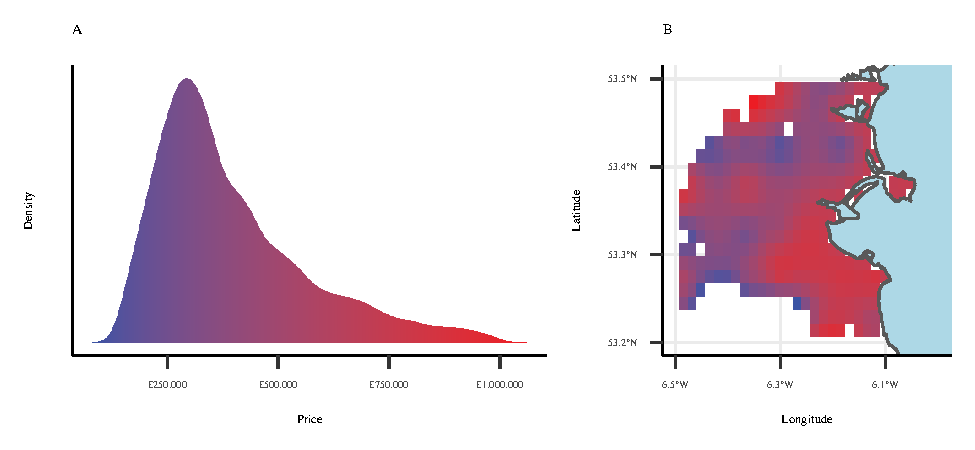
\includegraphics[width=0.98\textwidth]{dsaa_application_manuscript_files/figure-latex/distrib-plot-1} \caption{Overall (A) and geographic (B) distribution of the houses prices density in the city of Dublin in 2018. The geographic distribution was obtained by using a generalized additive model with soap film smooth parameter to take into account the influence of coastal boundaries. Geographic estimates outside of the 95\% Confidence Interval were removed.}\label{fig:distrib-plot}
\end{figure*}

The density of housing prices reveals a unimodal distribution of property prices (Figure \ref{fig:distrib-plot}A). In addition, the geographical distribution of property prices indicates a higher valuation in the South-West of the city as well as on the coast line (Figure \ref{fig:distrib-plot}B).

\hypertarget{correlates-with-urban-features}{%
\subsection{Correlates with urban features}\label{correlates-with-urban-features}}

Using the XGBoost algorithm, the 160 urban features are explaining 47\% of the property price variance (\(F(1, 2076) = 1,840.91\), \(p < .001\)) with a \(RMSE\) of €124,364 and a \(MAE\) of €83,963.61.

\begin{figure}
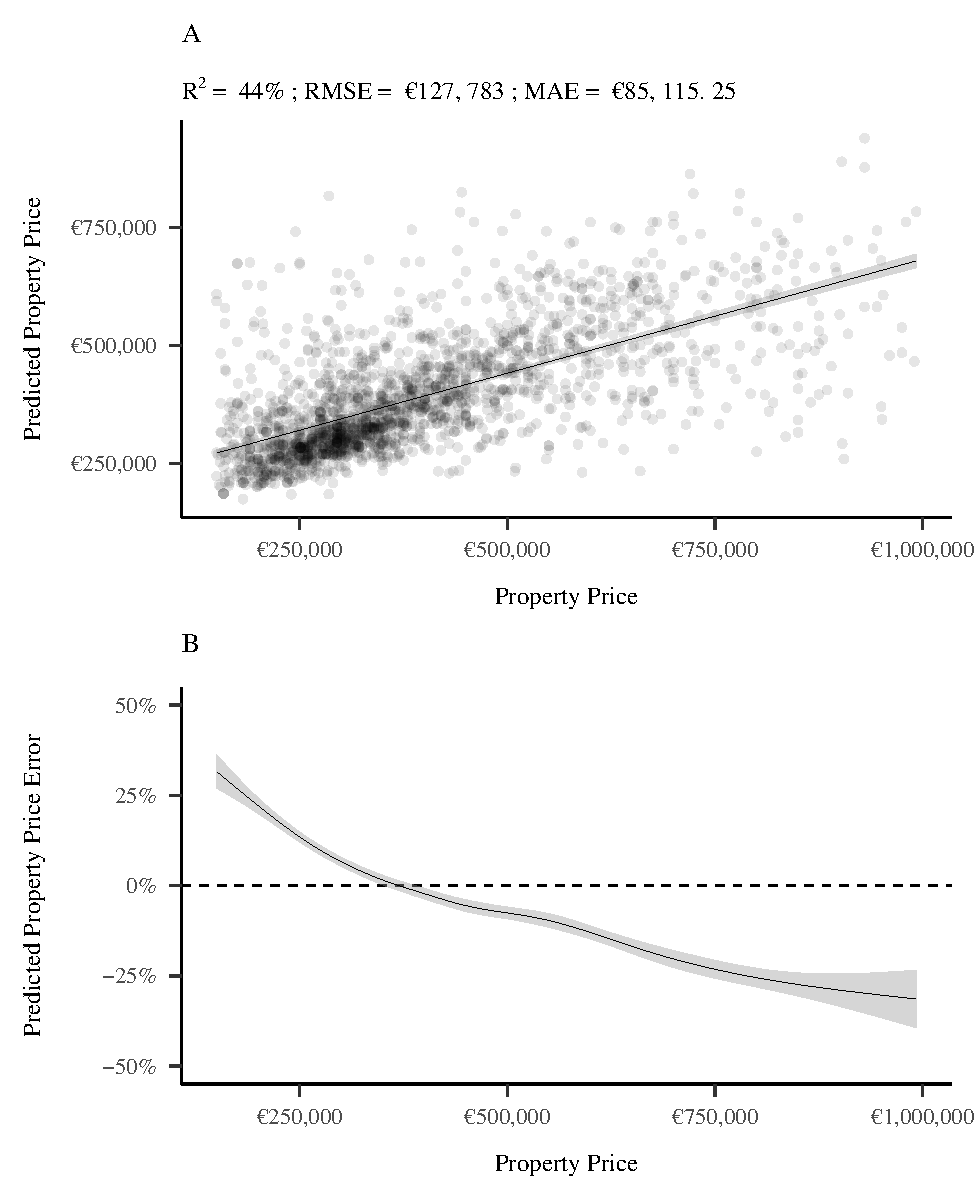
\includegraphics[width=0.98\columnwidth]{dsaa_application_manuscript_files/figure-latex/osm-features-xgb-1} \caption{Property price prediction accuracy (A) and Property price prediction error (B) using urban features with XGBoost.}\label{fig:osm-features-xgb}
\end{figure}

The overall correlation of the predicted property prices with urban features is shown in Figure \ref{fig:osm-features-xgb}A. It can be noticed that property prices situated at the low and the high end of the range are the most difficult to predict (Figure \ref{fig:osm-features-xgb}B). A possible explanation is the absence of distinctive and recurrent patterns in urban features for these houses. However, the prices higher than €300,000 are potentially driving down the prediction accuracy due to outliers.

\begin{table}

\caption{\label{tab:osm-features-table}Urban features importance (higher than 1\%).}
\centering
\fontsize{8}{10}\selectfont
\begin{tabu} to \linewidth {>{\raggedright}X>{\raggedright}X>{\raggedright}X}
\toprule
Feature Category & Feature Type & Importance\\
\midrule
amenity & embassy & 18.2\%\\
natural & grassland & 6.7\%\\
power & line & 2.3\%\\
route & bus & 2.2\%\\
boundary & administrative & 2.1\%\\
boundary & political & 1.7\%\\
route & ferry & 1.7\%\\
highway & residential & 1.3\%\\
highway & secondary & 1.2\%\\
historic & yes & 1.2\%\\
route & power & 1.1\%\\
cycleway & lane & 1.1\%\\
service & crossover & 1.1\%\\
barrier & wall & 1.1\%\\
place & locality & 1.1\%\\
area & yes & 1.0\%\\
\bottomrule
\end{tabu}
\end{table}

By analysing their importance (Table \ref{tab:osm-features-table}), the most relevant geographical features to predict housing prices are the distance to an embassy (18.2\%) and the distance to natural grasslands such as parks and gardens (6.7\%).

\hypertarget{correlates-with-socio-economic-features}{%
\subsection{Correlates with socio-economic features}\label{correlates-with-socio-economic-features}}

Using the XGBoost algorithm, the 48 socio-economic features explain 42\% of the property price variance (\(F(1, 2076) = 1,508.10\), \(p < .001\)) with a \(RMSE\) of €131,322 and a \(MAE\) of €87,328.79.

\begin{figure}
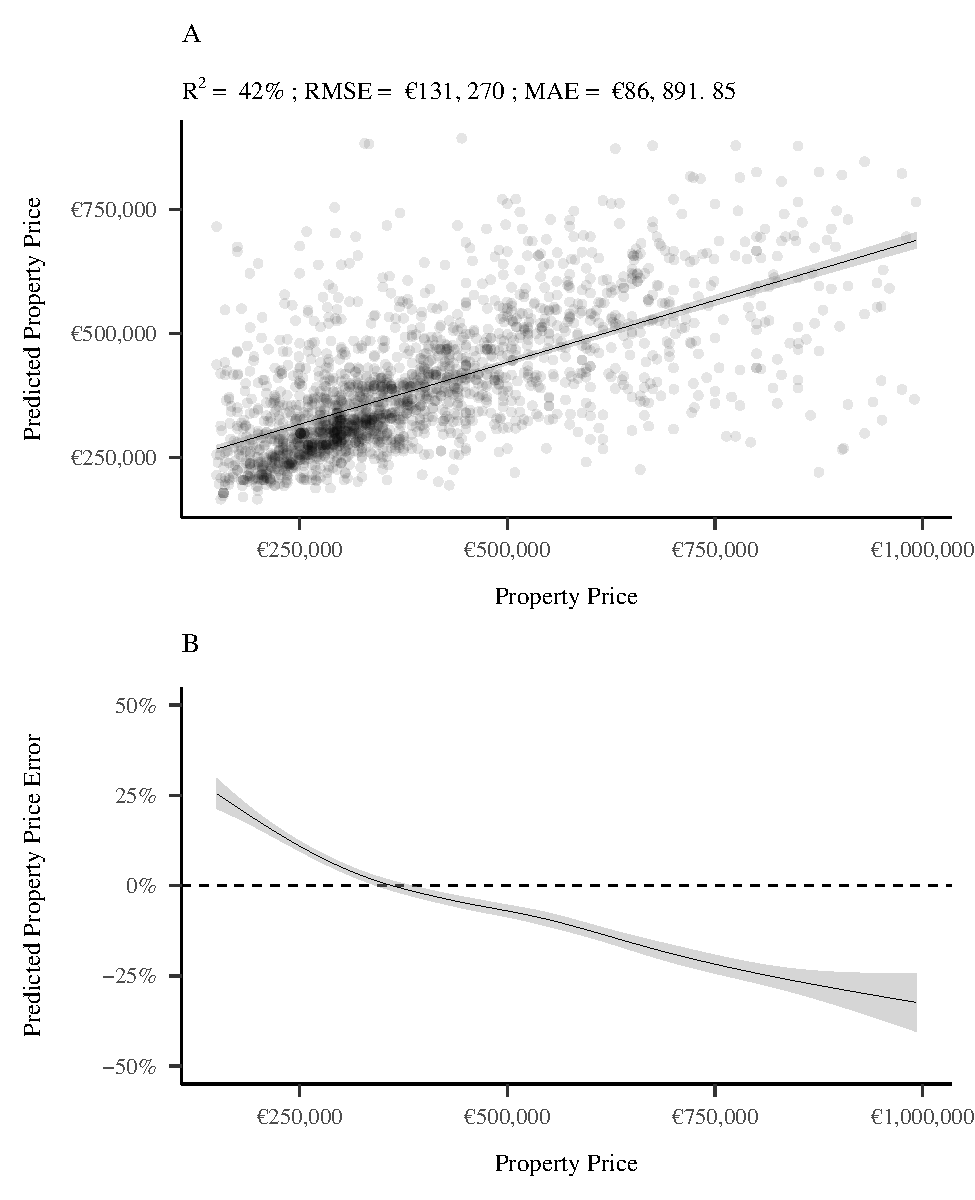
\includegraphics[width=0.98\columnwidth]{dsaa_application_manuscript_files/figure-latex/census-features-xgb-1} \caption{Property price prediction accuracy (A) and Property price prediction error (B) using socio-economic features with XGBoost.}\label{fig:census-features-xgb}
\end{figure}

The overall correlation of the predicted property prices with socio-economic features is shown in Figure \ref{fig:census-features-xgb}A. Similar to the model used for urban features, the model based on socio-economic features reveals that prices lower than €300,000 lead to the highest errors in over-valuation while prices higher than €300,000 lead to systematic under-valuation errors (Figure \ref{fig:census-features-xgb}B).

\begin{table}

\caption{\label{tab:census-features-table}Socio-economic features importance (higher than 1\%).}
\centering
\fontsize{8}{10}\selectfont
\begin{tabular}[t]{lll}
\toprule
Feature Category & Feature Type & Importance\\
\midrule
housing rooms & 8 or more Rooms & 29.0\%\\
religion & No Religion & 5.0\%\\
population & Age 0 - 14 & 3.8\%\\
housing rooms & 6 Rooms & 3.3\%\\
general health & Very Good & 3.1\%\\
population & Age 80 Plus & 2.8\%\\
housing tenure & Owner Occupier with Mortgage & 2.5\%\\
general health & Good & 2.4\%\\
religion & Other Catholic & 2.4\%\\
housing rooms & 5 Rooms & 2.3\%\\
disabilty age group & Persons with a disability aged 25 - 44 & 2.3\%\\
religion & No Answer & 2.2\%\\
housing rooms & 7 Rooms & 2.2\%\\
disabilty age group & Persons with a disability aged 0 - 14 & 2.0\%\\
population & Age 45 - 64 & 1.8\%\\
population & Age 15 - 24 & 1.6\%\\
disabilty age group & Persons with a disability aged 65 Plus & 1.6\%\\
housing rooms & 3 Rooms & 1.6\%\\
housing tenure & Social Rented & 1.6\%\\
disabilty age group & Persons with a disability aged 45 - 64 & 1.5\%\\
housing tenure & Rented Free of Rent & 1.4\%\\
disabilty age group & Persons with a disability aged 15 - 44 & 1.4\%\\
general health & Bad & 1.4\%\\
housing rooms & 1 Room & 1.4\%\\
housing tenure & Owner Occupier No Mortgage & 1.4\%\\
disabilty age group & Total persons with a disability & 1.2\%\\
housing rooms & 4 Rooms & 1.2\%\\
population & Female & 1.2\%\\
religion & Roman Catholic & 1.2\%\\
population & Age 25 - 44 & 1.1\%\\
carers & Provides No Care & 1.1\%\\
housing tenure & Private Rented & 1.0\%\\
\bottomrule
\end{tabular}
\end{table}

According to the analysis of the relative importance of socio-economic features (Table \ref{tab:census-features-table}), the most important socio-economic features are the proportion of large houses (i.e., houses with eight or more rooms) in the small area containing the property (29.0\%). It also appears that areas having a high proportion of young children (3.8\%), as well as the proportion of people reporting that they have no religion (5.0\%), influence the model.

\hypertarget{discussion}{%
\section{Discussion}\label{discussion}}

While Dublin is a very specific city due to its low population density spread on a large surface, its housing market is one of the most expensive in Europe. The main reason is the structure of the market, mainly made of residential properties and few apartment buildings. In this study, the prices of 10387 properties sold in 2018 in the area of Dublin were analysed from the Property Services Regulatory Authority database in order to identify the potential factors correlating with these prices. The enforcement of a housing price registry has been shown as being an essential tool to regulate the housing market (Tomson 2016). However, a major limitation of this study is the absence of characteristics for the property itself. Indeed, prices are mainly determined by factors such as the size of the property or the number of rooms.

Despite the absence of property characteristics, urban and socio-economic features were used to identify spatial correlates to the housing prices. Results revealed that proximity to embassies and grasslands is a driver of house prices. Embassies are in general located in the most expensive areas of cities which are also the most aesthetically pleasing and the most secure part of cities. In addition, the density of embassies and properties allocated to embassy staff reduces the density of property available on the market and drives their prices up. The distance to a park or a natural area is also a very important factor for house prices. Results also revealed that the density of large houses in the area and the proportion of individuals reporting having no religion are very important. Again, the size of the property sold was not included in the database; however, the higher the density of large houses in the area, the higher the probability for the property to be a large house. The second most important feature is the density of young children. While the literature is not conclusive of the link between wealth and family size, future research could investigate the mediation effect of house size between family size and property price. Finally, the relation with the expression of religious belief, or more precisely its absence, is a very interesting feature. Again, the relationship between religion and income is not confirmed by the literature. Whereas some studies reveal a positive correlation between religion and income (Guiso, Sapienza, and Zingales 2003; Elgin et al. 2013) others reveals no evidence of such relationship (De La O and Rodden 2008). Here, it appears that prices of houses are higher in areas with a high density of people indicating that they have no religion.

\hypertarget{conclusion}{%
\section{Conclusion}\label{conclusion}}

The evolution of housing prices is a pressing issue in most European capitals and specially in Dublin. Given their significant increase, houses are less and less affordable for individuals. By preforming a feature analysis with urban and socio-economic features, it is possible to evaluate and predict the potential price of a house. Indeed features such as the presence of embassies or parks are criteria that influence significantly the price of houses. Similarly, the characteristics of inhabitants in the area such as religion, health and age is correlated to the evolution of housing prices. These results allow an understanding of why some areas have higher prices than others.

\hypertarget{acknowledgement}{%
\section{Acknowledgement}\label{acknowledgement}}

The authors would like to thank the developers of the following R packages used to process, analyse, display and report data: R (Version 4.0.0; R Core Team 2020) and the R-packages \emph{dplyr} (Version 1.0.0; Wickham, François, et al. 2020), \emph{forcats} (Version 0.5.0; Wickham 2020), \emph{ggplot2} (Version 3.3.1; Wickham 2016), \emph{here} (Version 0.1; Müller 2017), \emph{kableExtra} (Version 1.1.0; Zhu 2019), \emph{latex2exp} (Version 0.4.0; Meschiari 2015), \emph{lubridate} (Version 1.7.8; Grolemund and Wickham 2011), \emph{lwgeom} (Version 0.2.4; Pebesma 2020), \emph{magrittr} (Version 1.5; Bache and Wickham 2014), \emph{mgcv} (Version 1.8.31; Wood 2011, 2004, 2003; Wood et al. 2016), \emph{nlme} (Version 3.1.147; Pinheiro et al. 2020), \emph{OpenStreetMap} (Version 0.3.4; Fellows and JMapViewer library by Jan Peter Stotz 2019), \emph{osmdata} (Version 0.1.3; Padgham et al. 2017), \emph{papaja} (Version 0.1.0.9942; Aust and Barth 2020), \emph{patchwork} (Version 1.0.0; Pedersen 2019), \emph{purrr} (Version 0.3.4; Henry and Wickham 2020), \emph{readr} (Version 1.3.1; Wickham, Hester, and Francois 2018), \emph{sf} (Version 0.9.3; Pebesma 2018), \emph{stringr} (Version 1.4.0; Wickham 2019), \emph{tibble} (Version 3.0.1; Müller and Wickham 2020), \emph{tidyr} (Version 1.1.0; Wickham and Henry 2020), \emph{tidyverse} (Version 1.3.0; Wickham, Averick, et al. 2019), \emph{tmap} (Version 3.0; Tennekes 2018), \emph{xgboost} (Version 1.0.0.2; Chen et al. 2020), and \emph{yardstick} (Version 0.0.6; Kuhn and Vaughan 2020).

\hypertarget{data-availability}{%
\section{Data availability}\label{data-availability}}

The R code and relevant data for statistical computing are available at https://github.com/damien-dupre/DSAA\_2020.

\hypertarget{references}{%
\section*{References}\label{references}}
\addcontentsline{toc}{section}{References}

\hypertarget{refs}{}
\leavevmode\hypertarget{ref-antonakakis2016dynamic}{}%
Antonakakis, Nikolaos, and Christos Floros. 2016. ``Dynamic Interdependencies Among the Housing Market, Stock Market, Policy Uncertainty and the Macroeconomy in the United Kingdom.'' \emph{International Review of Financial Analysis} 44: 111--22.

\leavevmode\hypertarget{ref-R-papaja}{}%
Aust, Frederik, and Marius Barth. 2020. \emph{papaja: Create APA Manuscripts with R Markdown}. \url{https://github.com/crsh/papaja}.

\leavevmode\hypertarget{ref-rppr2020}{}%
Authority, Property Services Regulatory. 2020. ``Residential Property Price Register.'' June 1, 2020. \url{https://propertypriceregister.ie}.

\leavevmode\hypertarget{ref-R-magrittr}{}%
Bache, Stefan Milton, and Hadley Wickham. 2014. \emph{Magrittr: A Forward-Pipe Operator for R}. \url{https://CRAN.R-project.org/package=magrittr}.

\leavevmode\hypertarget{ref-basu1998analysis}{}%
Basu, Sabyasachi, and Thomas G Thibodeau. 1998. ``Analysis of Spatial Autocorrelation in House Prices.'' \emph{The Journal of Real Estate Finance and Economics} 17 (1): 61--85.

\leavevmode\hypertarget{ref-bourassa2007spatial}{}%
Bourassa, Steven C, Eva Cantoni, and Martin Hoesli. 2007. ``Spatial Dependence, Housing Submarkets, and House Price Prediction.'' \emph{The Journal of Real Estate Finance and Economics} 35 (2): 143--60.

\leavevmode\hypertarget{ref-chen2016xgboost}{}%
Chen, Tianqi, and Carlos Guestrin. 2016. ``Xgboost: A Scalable Tree Boosting System.'' In \emph{Proceedings of the 22nd Acm Sigkdd International Conference on Knowledge Discovery and Data Mining}, 785--94.

\leavevmode\hypertarget{ref-R-xgboost}{}%
Chen, Tianqi, Tong He, Michael Benesty, Vadim Khotilovich, Yuan Tang, Hyunsu Cho, Kailong Chen, et al. 2020. \emph{Xgboost: Extreme Gradient Boosting}. \url{https://CRAN.R-project.org/package=xgboost}.

\leavevmode\hypertarget{ref-clapp2002predicting}{}%
Clapp, John M, Hyon--Jung Kim, and Alan E Gelfand. 2002. ``Predicting Spatial Patterns of House Prices Using Lpr and Bayesian Smoothing.'' \emph{Real Estate Economics} 30 (4): 505--32.

\leavevmode\hypertarget{ref-de2008does}{}%
De La O, Ana L, and Jonathan A Rodden. 2008. ``Does Religion Distract the Poor? Income and Issue Voting Around the World.'' \emph{Comparative Political Studies} 41 (4-5): 437--76.

\leavevmode\hypertarget{ref-dubin1998predicting}{}%
Dubin, Robin A. 1998. ``Predicting House Prices Using Multiple Listings Data.'' \emph{The Journal of Real Estate Finance and Economics} 17 (1): 35--59.

\leavevmode\hypertarget{ref-elgin2013religion}{}%
Elgin, Ceyhun, Turkmen Goksel, Mehmet Y Gurdal, and Cuneyt Orman. 2013. ``Religion, Income Inequality, and the Size of the Government.'' \emph{Economic Modelling} 30: 225--34.

\leavevmode\hypertarget{ref-R-OpenStreetMap}{}%
Fellows, Ian, and using the JMapViewer library by Jan Peter Stotz. 2019. \emph{OpenStreetMap: Access to Open Street Map Raster Images}. \url{https://CRAN.R-project.org/package=OpenStreetMap}.

\leavevmode\hypertarget{ref-feng2015comparing}{}%
Feng, Yingyu, and Kelvyn Jones. 2015. ``Comparing Multilevel Modelling and Artificial Neural Networks in House Price Prediction.'' In \emph{2015 2nd Ieee International Conference on Spatial Data Mining and Geographical Knowledge Services (Icsdm)}, 108--14. IEEE.

\leavevmode\hypertarget{ref-friedman2001greedy}{}%
Friedman, Jerome H. 2001. ``Greedy Function Approximation: A Gradient Boosting Machine.'' \emph{Annals of Statistics}, 1189--1232.

\leavevmode\hypertarget{ref-goodman1998housing}{}%
Goodman, Allen C, and Thomas G Thibodeau. 1998. ``Housing Market Segmentation.'' \emph{Journal of Housing Economics} 7 (2): 121--43.

\leavevmode\hypertarget{ref-R-lubridate}{}%
Grolemund, Garrett, and Hadley Wickham. 2011. ``Dates and Times Made Easy with lubridate.'' \emph{Journal of Statistical Software} 40 (3): 1--25. \url{http://www.jstatsoft.org/v40/i03/}.

\leavevmode\hypertarget{ref-guiso2003people}{}%
Guiso, Luigi, Paola Sapienza, and Luigi Zingales. 2003. ``People's Opium? Religion and Economic Attitudes.'' \emph{Journal of Monetary Economics} 50 (1): 225--82.

\leavevmode\hypertarget{ref-haklay2008openstreetmap}{}%
Haklay, Mordechai, and Patrick Weber. 2008. ``Openstreetmap: User-Generated Street Maps.'' \emph{IEEE Pervasive Computing} 7 (4): 12--18.

\leavevmode\hypertarget{ref-R-purrr}{}%
Henry, Lionel, and Hadley Wickham. 2020. \emph{Purrr: Functional Programming Tools}. \url{https://CRAN.R-project.org/package=purrr}.

\leavevmode\hypertarget{ref-R-yardstick}{}%
Kuhn, Max, and Davis Vaughan. 2020. \emph{Yardstick: Tidy Characterizations of Model Performance}. \url{https://CRAN.R-project.org/package=yardstick}.

\leavevmode\hypertarget{ref-limsombunchai2004house}{}%
Limsombunchai, Visit. 2004. ``House Price Prediction: Hedonic Price Model Vs. Artificial Neural Network.'' In \emph{New Zealand Agricultural and Resource Economics Society Conference}, 25--26.

\leavevmode\hypertarget{ref-liu2013spatial}{}%
Liu, Xiaolong. 2013. ``Spatial and Temporal Dependence in House Price Prediction.'' \emph{The Journal of Real Estate Finance and Economics} 47 (2): 341--69.

\leavevmode\hypertarget{ref-mccluskey2000application}{}%
McCluskey, William J, William G Deddis, Ian G Lamont, and Richard A Borst. 2000. ``The Application of Surface Generated Interpolation Models for the Prediction of Residential Property Values.'' \emph{Journal of Property Investment \& Finance}.

\leavevmode\hypertarget{ref-R-latex2exp}{}%
Meschiari, Stefano. 2015. \emph{Latex2exp: Use Latex Expressions in Plots}. \url{https://CRAN.R-project.org/package=latex2exp}.

\leavevmode\hypertarget{ref-R-here}{}%
Müller, Kirill. 2017. \emph{Here: A Simpler Way to Find Your Files}. \url{https://CRAN.R-project.org/package=here}.

\leavevmode\hypertarget{ref-R-tibble}{}%
Müller, Kirill, and Hadley Wickham. 2020. \emph{Tibble: Simple Data Frames}. \url{https://CRAN.R-project.org/package=tibble}.

\leavevmode\hypertarget{ref-cso2020}{}%
Office, Central Statistics. 2020. ``Census 2016 Small Area Population Statistics.'' June 1, 2020. \url{http://census.cso.ie/sapmap}.

\leavevmode\hypertarget{ref-openstreetmap2020}{}%
OpenStreetMap. 2020. ``Map Features (Wiki).'' June 1, 2020. \url{https://wiki.openstreetmap.org/wiki/Map_Features}.

\leavevmode\hypertarget{ref-R-osmdata}{}%
Padgham, Mark, Bob Rudis, Robin Lovelace, and Maëlle Salmon. 2017. ``Osmdata.'' \emph{The Journal of Open Source Software} 2 (14). \url{https://doi.org/10.21105/joss.00305}.

\leavevmode\hypertarget{ref-R-sf}{}%
Pebesma, Edzer. 2018. ``Simple Features for R: Standardized Support for Spatial Vector Data.'' \emph{The R Journal} 10 (1): 439--46. \url{https://doi.org/10.32614/RJ-2018-009}.

\leavevmode\hypertarget{ref-R-lwgeom}{}%
---------. 2020. \emph{Lwgeom: Bindings to Selected 'Liblwgeom' Functions for Simple Features}. \url{https://CRAN.R-project.org/package=lwgeom}.

\leavevmode\hypertarget{ref-R-patchwork}{}%
Pedersen, Thomas Lin. 2019. \emph{Patchwork: The Composer of Plots}. \url{https://CRAN.R-project.org/package=patchwork}.

\leavevmode\hypertarget{ref-R-nlme}{}%
Pinheiro, Jose, Douglas Bates, Saikat DebRoy, Deepayan Sarkar, and R Core Team. 2020. \emph{nlme: Linear and Nonlinear Mixed Effects Models}. \url{https://CRAN.R-project.org/package=nlme}.

\leavevmode\hypertarget{ref-R-base}{}%
R Core Team. 2020. \emph{R: A Language and Environment for Statistical Computing}. Vienna, Austria: R Foundation for Statistical Computing. \url{https://www.R-project.org/}.

\leavevmode\hypertarget{ref-savage2014property}{}%
Savage, Michael, James Barlow, Peter Dickens, and Tom Fielding. 2014. \emph{Property Bureaucracy \& Culture}. Routledge.

\leavevmode\hypertarget{ref-selim2009determinants}{}%
Selim, Hasan. 2009. ``Determinants of House Prices in Turkey: Hedonic Regression Versus Artificial Neural Network.'' \emph{Expert Systems with Applications} 36 (2): 2843--52.

\leavevmode\hypertarget{ref-R-tmap}{}%
Tennekes, Martijn. 2018. ``tmap: Thematic Maps in R.'' \emph{Journal of Statistical Software} 84 (6): 1--39. \url{https://doi.org/10.18637/jss.v084.i06}.

\leavevmode\hypertarget{ref-tomson2016property}{}%
Tomson, AIVAR. 2016. ``Property Sales Register as a Tool to Improve the Quality of Valuation and Market Research: Lessons Learned from Selected Countries.'' In \emph{World Bank Conference on Land and Poverty, Washington, Dc, March}, 14--18.

\leavevmode\hypertarget{ref-R-ggplot2}{}%
Wickham, Hadley. 2016. \emph{Ggplot2: Elegant Graphics for Data Analysis}. Springer-Verlag New York. \url{https://ggplot2.tidyverse.org}.

\leavevmode\hypertarget{ref-R-stringr}{}%
---------. 2019. \emph{Stringr: Simple, Consistent Wrappers for Common String Operations}. \url{https://CRAN.R-project.org/package=stringr}.

\leavevmode\hypertarget{ref-R-forcats}{}%
---------. 2020. \emph{Forcats: Tools for Working with Categorical Variables (Factors)}. \url{https://CRAN.R-project.org/package=forcats}.

\leavevmode\hypertarget{ref-R-tidyverse}{}%
Wickham, Hadley, Mara Averick, Jennifer Bryan, Winston Chang, Lucy D'Agostino McGowan, Romain François, Garrett Grolemund, et al. 2019. ``Welcome to the tidyverse.'' \emph{Journal of Open Source Software} 4 (43): 1686. \url{https://doi.org/10.21105/joss.01686}.

\leavevmode\hypertarget{ref-R-dplyr}{}%
Wickham, Hadley, Romain François, Lionel Henry, and Kirill Müller. 2020. \emph{Dplyr: A Grammar of Data Manipulation}. \url{https://CRAN.R-project.org/package=dplyr}.

\leavevmode\hypertarget{ref-R-tidyr}{}%
Wickham, Hadley, and Lionel Henry. 2020. \emph{Tidyr: Tidy Messy Data}. \url{https://CRAN.R-project.org/package=tidyr}.

\leavevmode\hypertarget{ref-R-readr}{}%
Wickham, Hadley, Jim Hester, and Romain Francois. 2018. \emph{Readr: Read Rectangular Text Data}. \url{https://CRAN.R-project.org/package=readr}.

\leavevmode\hypertarget{ref-wood2008soap}{}%
Wood, Simon N, Mark V Bravington, and Sharon L Hedley. 2008. ``Soap Film Smoothing.'' \emph{Journal of the Royal Statistical Society: Series B (Statistical Methodology)} 70 (5): 931--55.

\leavevmode\hypertarget{ref-R-mgcv_d}{}%
Wood, S. N. 2003. ``Thin-Plate Regression Splines.'' \emph{Journal of the Royal Statistical Society (B)} 65 (1): 95--114.

\leavevmode\hypertarget{ref-R-mgcv_c}{}%
---------. 2004. ``Stable and Efficient Multiple Smoothing Parameter Estimation for Generalized Additive Models.'' \emph{Journal of the American Statistical Association} 99 (467): 673--86.

\leavevmode\hypertarget{ref-R-mgcv_a}{}%
---------. 2011. ``Fast Stable Restricted Maximum Likelihood and Marginal Likelihood Estimation of Semiparametric Generalized Linear Models.'' \emph{Journal of the Royal Statistical Society (B)} 73 (1): 3--36.

\leavevmode\hypertarget{ref-R-mgcv_b}{}%
Wood, S. N., N., Pya, and B. S"afken. 2016. ``Smoothing Parameter and Model Selection for General Smooth Models (with Discussion).'' \emph{Journal of the American Statistical Association} 111: 1548--75.

\leavevmode\hypertarget{ref-R-kableExtra}{}%
Zhu, Hao. 2019. \emph{KableExtra: Construct Complex Table with 'Kable' and Pipe Syntax}. \url{https://CRAN.R-project.org/package=kableExtra}.

\end{document}


